\section[Properties of 3 variable quasi-invariants]{Properties of $\boldsymbol{3}$ variable quasi-invariants}\label{sec:wang}
Similarly to the $p=2$ case, we can adapt many of the properties of $Q_m(3,\mathbf{F}_p)$ for $p>3$ found in \cite{wang2022explicit} to the $p=3$ case. We accomplish this by converting $\std$ to $\siv$. For example, in~$Q_0(3,\mathbf{F}_p)$ for $p>3$, the space spanned by $x_1-x_2$, $x_1-x_3$ is a copy of $\std$. However, in~$Q_0(3,\mathbf{F}_3)$, the space spanned by $x_1-x_2$, $x_1-x_3$ becomes a copy of $\siv$. Using this, we may show that there are equivalents of Lemmas 3.2--3.5 from \cite{wang2022explicit} in characteristic~$3$.

We define $V_{i_1i_2}^{-}$ to be the $(-1)$-eigenspace of $s_{i_1i_2}$ in $V$, where $V$ is a copy of $\std$ or $\siv$. Note that if $v\in V_{i_1i_2}^{-}$ we have $v=s_{23}v+s_{13}v$. The following lemma and corollary correspond to Lemma~3.2 and Corollary~3.3 from \cite{wang2022explicit}, respectively.

\begin{Lemma}\label{lem:3.1}
 Let $V$ be a copy of $\siv$ in $Q_m(3,\mathbf{F}_3)_{\siv}$, and let $K\in V_{i_1i_2}^{-}$. Then we have $K+sK+s^2K=0$, where $s=(1\,2\,3)\in S_3$ and $K=(x_{i_1}-x_{i_2})^{2m+1}K'$ for some polynomial~$K'$ that is invariant under the action of $s_{i_1i_2}$. Conversely, let $K'$ be an $s_{12}$-invariant polynomial such that
 \[(x_1-x_2)^{2m+1}K'+(x_2-x_3)^{2m+1}sK'+(x_3-x_1)^{2m+1}s^2K'=0.\]
 Then $(x_1-x_2)^{2m+1}K'$ either belongs to $Q_m(3,\mathbf{F}_3)_\sign$ or the $(-1)$-eigenspace of $s_{12}$ in some copy of $\siv$ inside $Q_m(3,\mathbf{F}_3)_\siv$.
\end{Lemma}

\begin{proof}
 The proof is largely the same as in \cite{wang2022explicit}; the only difference is in the last step. Namely, now we have 2 2-dimensional indecomposable representations $\siv$ and $\tign$, but an~element in the $(-1)$-eigenspace of $s_{12}$ in $\tign$ must be in a copy of $\sign$.
\end{proof}

\begin{Corollary}\label{cor:3.2}
 Let $K$ be a generator of $Q_m(3,\mathbf{F}_3)_\siv$ in $V_{i_1i_2}^-$ for some copy $V$ of $\siv$ and write $K=(x_{i_1}-x_{i_2})^{2m+1}K'$. Then $K'$ is not divisible by any nonconstant symmetric polynomial.
\end{Corollary}

The proof of this corollary is identical to the proof of \cite[Corollary 3.3]{wang2022explicit}.

We define generators of $Q_m(3,\mathbf{F}_3)$ to be ``distinct'' if they are either in different degrees, or if no linear combination of them over $\mathbf{F}_3$ is generated by lower degree generators.

\begin{Lemma}\label{lem:3.3}
 Let $K$ and $L$ be distinct generators of $Q_m(3,\k)_\siv$, and let $V$ and $W$ be the~copies of $\siv$ generated by $K$ and $L$ respectively such that $K\in V_{i_1i_2}^{-}$ and $L\in W_{i_1i_2}^{-}$. Then $Ks_{23}L - Ls_{23}K$ is a nonzero element of $Q_m(3,\mathbf{F}_3)_{\sign}$ and $\deg V+\deg W\geq 6m+3$.
\end{Lemma}

Noting that $\wedge^2(\siv) = \sign$, the proof of this lemma is also identical to the proof of~\mbox{\cite[Lemma 3.4]{wang2022explicit}}.

Lemma 3.5 from \cite{wang2022explicit} does not completely hold in characteristic $3$. A very similar and useful version does, however, and we have the following.

\begin{Lemma}\label{lem:3.4}
 Assume that there exists generators $K$ and $L$ of $Q_m(3,\mathbf{F}_3)_\siv$ such that $\deg K+\deg L=6m+3$. Then $Q_m(3,\mathbf{F}_3)_\siv$ is freely generated by $K$, $L$, and $1$ over $\mathbf{F}_3[x_1,x_2,x_3]^{S_3}$.
\end{Lemma}
\begin{proof}
 We note that $(L+s_{23}L)K-(K+s_{23}K)L=c\prod_{i_1<i_2}(x_{i_1}-x_{i_2})^{2m+1}$ for some $c\neq 0$ by Lemma~\ref{lem:3.3}. Moreover, $L+s_{23}L$ and $K+s_{23}K$ are symmetric because $K$ and $L$ are both acted on by negation by $s_{12}$, so elements in $Q_m(3,\mathbf{F}_3)_{\sign}$ are generated by $K$ and $L$. From there, the fact that $Q_m(3,\mathbf{F}_3)_\siv$ is generated by $K$, $L$, and $1$ over $\mathbf{F}_3[x_1,x_2,x_3]^{S_3}$ follows from the first part of the proof from \cite{wang2022explicit}.

 To prove freeness, assume for the sake of contradiction that there was a relation $PK+QL+S=0$ for symmetric polynomials $P$, $Q$, and $S$. $PK$ and $QL$ are both in the $(-1)$-eigenspace of $s_{12}$ while $S$ is not, so $S=0$. Thus we have $PK=-QL$ and from there we can proceed the same as \cite{wang2022explicit}.

\end{proof}

\section{Ren--Xu counterexamples}\label{sec:renxu}

We aim to explicitly describe the Hilbert series of $Q_m(3,\mathbf{F}_3)$. To do so we wish to identify the generators of $Q_m(3,\mathbf{F}_3)_{\siv}$.

In \cite{Ren_2020}, Ren and Xu found polynomials of the form $P_k^{3^a}\prod (x_{i_1}-x_{i_2})^{2b}$ in $Q_m(3,\mathbf{F}_3)$ with degree strictly less than $3m+1$, where $P_k$ is the map of the $3k+1$ degree generator of $Q_k(3,\mathbf{Q})$ into characteristic $3$ and where $a$, $k$, and $b$ are natural numbers. We refer to these polynomials as Ren--Xu counterexamples as they demonstrate the Hilbert series of $Q_m(3,\mathbf{F}_3)$ differs from that of $Q_m(3,\mathbf{Q})$ for certain $m$.

\begin{Definition}
 Let $\overline{P_k}$ be the generator of $Q_k(3,\mathbf{Q})$ of degree $3k+1$ in the $(-1)$-eigenspace of $s_{12}$, expressed as an integer polynomial with coprime coefficients. Let $P_k$ be the image of $\overline{P_k}$ under the quotient map $\Z[x_1,x_2,x_3]\to\F_3[x_1,x_2,x_3]$. Define the set $X$ as the set of all natural numbers $m$ such that $Q_m(3,\mathbf{F}_3)$ has a Ren--Xu counterexample. Let $R_m$ be a lowest degree Ren--Xu counterexample in $Q_m(3,\mathbf{F}_3)$ for all $m\in X$.
\end{Definition}


A key step in describing the Hilbert series of $Q_m(3,\mathbf{F}_3)$ is proving Ren--Xu's conjecture~\cite{Ren_2020} for ${n=3}$ and~${p=3}$.

\begin{Conjecture}[\cite{Ren_2020}]\label{conj:ren}
 If the Hilbert series of $Q_m(n,\mathbf{F}_p)$ differs from that of $Q_m(n,\mathbf{Q})$, then there exists integers $a\geq 0$ and $k\geq 0$ such that
 \[\frac{mn(n-2)+\binom{n}{2}}{n(n-2)k+\binom{n}{2}-1}\leq p^a\leq \frac{mn}{nk+1}.\]
\end{Conjecture}

The main step for proving the conjecture for $n=3$, $p=3$ is the following theorem.

\begin{Theorem}\label{justRens}
 $Q_m(3,\mathbf{F}_3)_{\siv}$ is either freely generated by a generator of degree $3m+1$, $3m+2$, and the polynomial $1$, or it is freely generated by $R_m$, another generator in degree $6m+3-\deg R_m$, and the polynomial $1$.
\end{Theorem}

To prove this theorem, we first describe the Ren--Xu counterexamples.

\begin{Lemma}\label{nonExsOnly}
 If $m\in X$, we must have $R_m=P_k^{3^a}\prod (x_{i_1}-x_{i_2})^{2b}$, where $a$, $b$, $k$ are natural numbers and $k\not \in X$.
\end{Lemma}
\begin{proof}
 Assume for contradiction that there exists a nonnegative integer $m\in X$ such that $R_m=P_k^{3^a}\prod (x_{i_1}-x_{i_2})^{2b}$, where $a$, $b$, $k$ are natural numbers and $k\in X$. Then if $R_k=P_{l}^{3^c}\prod (x_{i_1}-x_{i_2})^{2d}$, the polynomial
 \[{R_k}^{3^a}\prod (x_{i_1}-x_{i_2})^{2b} = P_{l}^{3^{a+c}}\prod (x_{i_1}-x_{i_2})^{2d\cdot 3^a + 2b}\]
 has a strictly smaller degree than $R_m$ since $\deg R_k<3k+1=\deg P_k$. Moreover, it is at least $m$-quasi-invariant, so it is a Ren--Xu counterexample for $Q_m(3,\mathbf{F}_3)$. Yet $R_m$ is a minimal counterexample, giving a contradiction.
\end{proof}

This lemma allows us to consider only counterexamples $P_k^{3^a}\prod (x_{i_1}-x_{i_2})^{2b}$ such that $Q_k(3,\mathbf{F}_3)$ does not contain a Ren--Xu counterexample.

From \cite{Ren_2020}, the Hilbert series for $Q_m(3,\mathbf{F}_3)$ differs from characteristic $0$ when there exists $a\in \mathbf{N}_0$ such that
\[\frac{1}{3}\leq \Bigl\{\frac{m}{3^a}\Bigr\}\leq \frac{2}{3}-\frac{1}{3^a}.\]
Notice this is equivalent to $m \pmod{3^a}$ being in $\bigl\{3^{a-1},3^{a-1}+1,\dots,2\cdot 3^{a-1}-1\bigr\}$.

\begin{Lemma} \label{noOnes}
 If $m\not\in X$, then the base $3$ representation of $m$ contains no $1$'s.
\end{Lemma}
\begin{proof}
 Suppose $m$ had the digit $1$ in the $a$-th position from the right. Then $m\pmod{3^a}$ has a~leading digit of $1$ if we choose $m\pmod{3^a}$ to be between $0$ and $3^a-1$ inclusive. However, this implies that $m \pmod{3^a}$ is in $\bigl\{3^{a-1},3^{a-1}+1,\dots,2\cdot 3^{a-1}-1\bigr\}$, so $m$ is a counterexample.
\end{proof}

\begin{Corollary}\label{evenCounter}
 If $m\not\in X$, then $m$ is even.
\end{Corollary}
\begin{proof}
 From Lemma~\ref{noOnes} $m$ has no $1$'s in its base $3$ representation, so
 \[m=\sum_{j=0}c_j3^j,\]
 where $c_j$ is $0$ or $2$. Thus $m$ must be even.
\end{proof}

\begin{Corollary}\label{noConsec}
 For all $m\not\in X$, we have $m+1\in X$.
\end{Corollary}
\begin{proof}
 By Corollary~\ref{evenCounter}, if $m\not\in X$, $m$ is even. Then $m+1$ is odd, so by the contrapositive of Corollary~\ref{evenCounter}, $m+1\in X$.
\end{proof}

Now we begin describing the degrees of Ren--Xu counterexamples.

\begin{Lemma} \label{countEx3m+3}
 If $Q_m(3,\mathbf{F}_3)_{\siv}$ has a generator in degree $3m+1$, then $m+1\in X$ and $\deg R_{m+1}=3m+3$.
\end{Lemma}
\begin{proof}
 If $m\in X$, we must have $\deg R_m<3m+1$. This implies a generator in a degree less than $3m+1$, violating Lemma~\ref{lem:3.3}. Thus $m\not\in X$, implying that $m+1\in X$ by Corollary~\ref{noConsec}.

 Because $\deg R_{m+1}<3m+4$ and $Q_{m+1}(3,\mathbf{F}_3)_\siv\subset Q_{m}(3,\mathbf{F}_3)_\siv$, we have $3m+1\leq\deg R_{m+1}< 3m+4$. By construction $3|\deg R_{m+1}$, so $\deg R_{m+1}= 3m+3$.
\end{proof}

We now introduce a few useful lemmas.

\begin{Lemma}\label{notInm+1}
 Suppose $Q_m(3,\mathbf{F}_3)_{\siv}$ has a smallest degree generator $L$ in degree $3m+1$. Assume that for all $j<m$, if $j\not\in X$, then $Q_j(3,\mathbf{F}_3)_\siv$ has a degree $3j+1$ generator. Then $Q_{m+1}(3,\mathbf{F}_3)_{\siv}$ has no nonsymmetric degree $3m+1$ or $3m+2$ element.
\end{Lemma}
\begin{proof}
 Any nonsymmetric $3m+1$ degree element in $Q_{m+1}(3,\mathbf{F}_3)_{\siv}$ must be a scalar multiple of $L$, so assume for contradiction $L$ is in $Q_{m+1}(3,\mathbf{F}_3)$. By Lemma~\ref{countEx3m+3}, $R_{m+1}=P_k^{3^a}\prod(x_{i_1}-x_{i_2})^{2b}$ is in degree $3m+3$ for natural numbers $a$, $b$, $k$. By Lemma~\ref{nonExsOnly}, $k\not\in X$ implying $P_k$ is a $3k+1$ generator of $Q_k(3,\mathbf{F}_3)_{\siv}$ using our assumption. Moreover, with any other generator in a degree less than $3m+3$ violating Lemma~\ref{lem:3.3}, $R_{m+1}$ must be generated by $L$, so $P_k^{3^a}\prod(x_{i_1}-x_{i_2})^{2b}=SL$ for some degree $2$ symmetric polynomial $S$. A degree $2$ symmetric polynomial divisible by $(x_{i_1}-x_{i_2})$ is impossible, so $S|P_k^{3^a}$ which implies either $S|P_k$ or $(x_1+x_2+x_3)|P_k$. Since $\overline{P_{k}}$ is in the $(-1)$-eigenspace of $s_{12}$, $P_{k}$ is as well and by Lemma~\ref{lem:3.1} we have $P_k=P_k'(x_1-x_2)^{2k+1}$. In both cases either $S|P_k'$ or $(x_1+x_2+x_3)|P_k'$. However, by our assumption $P_k$ is a generator, so $P_k'$ is not divisible by any nonconstant symmetric polynomial by Corollary~\ref{cor:3.2}.

 Similarly, suppose for contradiction that $K$ is a nonsymmetric element of $Q_{m+1}(3,\mathbf{F}_3)_{\siv}$ of degree $3m+2$. Since $Q_{m+1}(3,\mathbf{F}_3)_{\siv}$ has no nonsymmetric $3m+1$ degree element, $K$ must be a generator. By Lemma~\ref{lem:3.3}, $K$ is the only generator in degree less than $3m+3$, so $P_k^{3^a}\prod(x_{i_1}-x_{i_2})^{2b}$ is a symmetric polynomial multiple of $K$. However, the only symmetric polynomials of degree $1$ are multiples of $x_1+x_2+x_3$, implying $(x_1+x_2+x_3)|P_k$ which is impossible by Corollary~\ref{cor:3.2}.
\end{proof}

Note that by \cite{felder2001action}, $Q_m(3,\mathbf{Q})_{\std}$ has generators in degree $3m+1$ and $3m+2$, and by \cite{wang2022explicit}, such generators with even degree are divisible by $x_1+x_2-2x_3$. Let $\pi$ be the canonical mapping from characteristic $0$ to characteristic $3$. We then have the following lemma.

\begin{Lemma}\label{3m+2}
 Suppose $Q_m(3,\mathbf{F}_3)_{\siv}$ has a generator $L$ in degree $3m+1$. We can choose the generators of $Q_m(3,\mathbf{Q})_{\std}$ to be integer polynomials $L'$ and $(x_1+x_2-2x_3)K'$ with $\pi(K')=\pi(L')=L$. Moreover, if
 \[G=(x_1+x_2+x_3)\biggl(\frac{K'-L'}{3}\biggr)-x_3K',\]
 then
 \[\pi(G)= (x_1+x_2+x_3)\pi\biggl(\frac{K'-L'}{3}\biggr)-x_3L\]
 is a degree $3m+2$ generator for $Q_m(3,\mathbf{F}_3)_{\siv}$.
\end{Lemma}
\begin{proof}
 Let $L'$ be an arbitrary $3m+1$ degree generator of $Q_m(3,\mathbf{Q})_{\std}$ with coprime integer coefficients in the $(-1)$-eigenspace of $s_{12}$. By Lemma~\ref{lem:3.1}, $\pi(L')$ is an element of the $(-1)$-eigenspace of $s_{12}$ in $Q_m(3,\mathbf{F}_3)_{\siv}$ and if $\pi(L')$ is not a scalar multiple of $L$ then there must exist some other generator of $Q_m(3,\mathbf{F}_3)_{\siv}$ with degree less than or equal to $3m+1$. That generator and $L$ would violate Lemma~\ref{lem:3.3}, so we may set $\pi(L')=L$.

 A higher degree generator of $Q_m(3,\mathbf{Q})_{\std}$ has degree $3m+2$. With $\deg L=3m+1$ implying $m\not\in X$, $3m+2$ is even by Corollary~\ref{evenCounter}. Using \cite{wang2022explicit}, we let $(x_1+x_2-2x_3)K'$ be an arbitrary degree $3m+2$ generator for $Q_m(3,\mathbf{Q})_{\std}$ with coprime integer coefficients. Similarly, $\pi((x_1+x_2-2x_3)K')= (x_1+x_2+x_3)\pi(K')$ is an element of $Q_m(3,\mathbf{F}_3)_{\siv}$, so $\pi(K')$ is a non-symmetric polynomial of degree $3m+1$ in $Q_m(3,\mathbf{F}_3)_\siv$. Thus it must be a scalar multiple of $L$, and we may set $\pi(K')=L$.

 Let $G=(x_1+x_2+x_3)\big(\frac{K'-L'}{3}\big)-x_3K'$. Since
 \[(x_1+x_2-2x_3)K'-(x_1+x_2+x_3)L' = (x_1+x_2+x_3)\big(K'-L'\big)-3x_3K'\]
 and $\pi(K'-L')=L-L=0$, we have $G\in Q_m(3,\mathbf{Q})\cap \mathbf{Z}[x_1,x_2,x_3]$. Then
 \[\pi(G)= (x_1+x_2+x_3)\pi\biggl(\frac{K'-L'}{3}\biggr)-x_3L.\]
 If $\pi(G)$ generated by $L$, we must have $\pi(G)=c(x_1+x_2+x_3)L$ for some $c\in \mathbf{F}_3$ since $\deg\left(\pi(G)\right)=\deg(L)+1$. However, $x_1+x_2+x_3$ does not divide $x_3L$ since $L$ is a generator, so $x_1+x_2+x_3\nmid \pi(G)$. Then if $\pi(G)$ was not a generator, there must be some generator other than $L$ for $Q_m(3,\mathbf{F}_3)$ in degree less than $3m+2$ which violates Lemma~\ref{lem:3.3}. Thus, $\pi(G)$ is a generator.
\end{proof}

We aim to prove that minimum Ren--Xu counterexamples are generators and represent the only cases, where the Hilbert series of the quasi-invariants differs between characteristics $0$ and~$3$. To this end, we describe the degree of Ren--Xu counterexamples.

\begin{Example}
 We notice a ``staircase'' pattern for Ren--Xu counterexamples. The following are counterexamples for $m=3,4,5$:
 \begin{gather*}
 (x_1-x_2)^9, \qquad (x_1-x_2)^9,\qquad
 (x_1-x_2)^9\prod (x_{i_1}-x_{i_2})^2.
 \end{gather*}
 We note that since $(x_1-x_2)^9\in Q_4(3,\mathbf{F}_3)$, $(x_1-x_2)^9$ is the Ren--Xu counterexample for both~${m=3}$ and $m=4$. Moreover, the counterexample in $Q_5(3,\mathbf{F}_3)$ is the previous counterexample $(x_1-x_2)^9$ multiplied by $\prod (x_{i_1}-x_{i_2})^2$ to add the extra factor of $(x_1-x_2)^2$. In~this way the degree of counterexample stays constant for the first half of the ``staircase'' and climbs by $6$ per each increase in $m$ thereafter. Moreover, we note that $m=2,6\not\in X$, so our ``staircase'' is surrounded by non-counterexamples. One can also compute another generator for $m=3, 4, 5$ in degree $12$, $18$, and $18$ respectively. Since $9+12=6\cdot 3+3$, $9+18=6\cdot 4+3$, and $15+18=6\cdot 5 +3$, $Q_m(3,\mathbf{F}_3)_{\siv}$ is freely generated by each of these generators and $1$ by Lemma~\ref{lem:3.4}. This way we see that the upper degree generators form a complement to the lower degree ones, climbing by $6$ degrees initially and staying constant for the second half of the staircase.

 Visually, the following figure shows the degree of the generators for $Q_m(3,\mathbf{F}_3)$ with respect to $m$ were the staircase pattern and Theorem~\ref{justRens} to hold.
 \begin{figure}[ht]%\label{fig1}
 \centering
 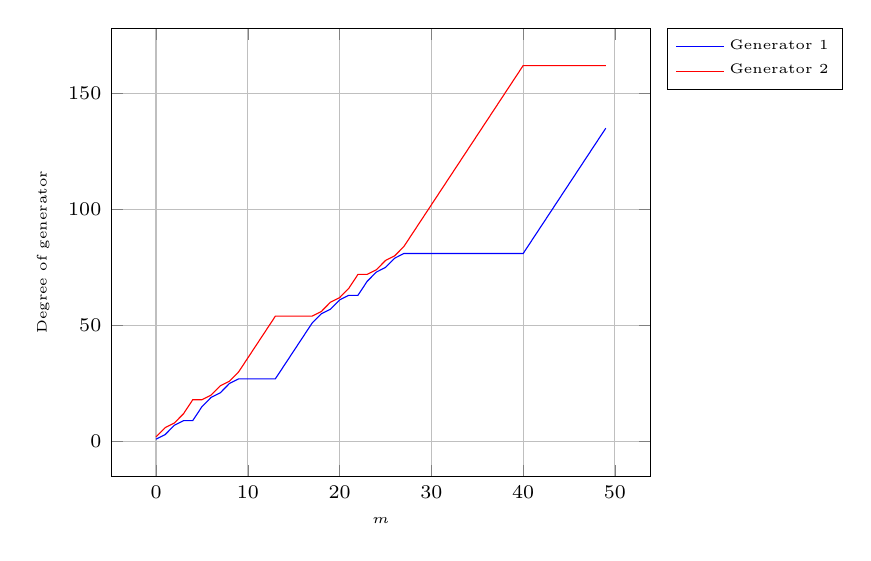
\begin{tikzpicture}[scale=1]
 \begin{axis}[
 tick label style={font=\scriptsize},
 xlabel={\tiny $m$},
 ylabel={\tiny Degree of generator},
 legend pos=outer north east,
 grid=major
 ]
 % Plot Lower values
 \addplot[color=blue] coordinates {
 (0,1)
 (1,3.0)
 (2,7)
 (3,9)
 (4,9.0)
 (5,15.0)
 (6,19)
 (7,21.0)
 (8,25)
 (9,27)
 (10,27)
 (11,27)
 (12,27)
 (13,27.0)
 (14,33.0)
 (15,39.0)
 (16,45.0)
 (17,51.0)
 (18,55)
 (19,57.0)
 (20,61)
 (21,63)
 (22,63.0)
 (23,69.0)
 (24,73)
 (25,75.0)
 (26,79)
 (27,81)
 (28,81)
 (29,81)
 (30,81)
 (31,81)
 (32,81)
 (33,81)
 (34,81)
 (35,81)
 (36,81)
 (37,81)
 (38,81)
 (39,81)
 (40,81.0)
 (41,87.0)
 (42,93.0)
 (43,99.0)
 (44,105.0)
 (45,111.0)
 (46,117.0)
 (47,123.0)
 (48,129.0)
 (49,135.0)
 };
 \addlegendentry{\tiny Generator $1$}

 % Plot Higher values
 \addplot[color=red] coordinates {
 (0,2)
 (1,6.0)
 (2,8)
 (3,12)
 (4,18.0)
 (5,18.0)
 (6,20)
 (7,24.0)
 (8,26)
 (9,30)
 (10,36)
 (11,42)
 (12,48)
 (13,54.0)
 (14,54.0)
 (15,54.0)
 (16,54.0)
 (17,54.0)
 (18,56)
 (19,60.0)
 (20,62)
 (21,66)
 (22,72.0)
 (23,72.0)
 (24,74)
 (25,78.0)
 (26,80)
 (27,84)
 (28,90)
 (29,96)
 (30,102)
 (31,108)
 (32,114)
 (33,120)
 (34,126)
 (35,132)
 (36,138)
 (37,144)
 (38,150)
 (39,156)
 (40,162.0)
 (41,162.0)
 (42,162.0)
 (43,162.0)
 (44,162.0)
 (45,162.0)
 (46,162.0)
 (47,162.0)
 (48,162.0)
 (49,162.0)
 };
 \addlegendentry{\tiny Generator $2$}

 \end{axis}
 \end{tikzpicture}
 \caption{Degrees of generators in characteristic $3$ with respect to $m$.} %\label{fig:enter-label}
\end{figure}
\end{Example}

 We prove that Ren--Xu counterexamples follow this staircase pattern.

\begin{Lemma}\label{staircase}
 Let $m$ be a natural number not in $X$ and let $d$ be the largest integer such that $R_{m+1}$ lies in $Q_{m+d}(3,\mathbf{F}_3)$. Suppose that for all $k\leq m$, if $k\not\in X$, then $Q_k(3,\mathbf{F}_3)_\siv$ has a generator in degree $3k+1$. Then $R_{m+j}=R_{m+1}$ in degree $3m+3$ for $1\leq j\leq d$ and $R_{m+j}=R_{m+1}\prod (x_{i_1}-x_{i_2})^{2(j-d)}$ in degree $3m+3+6(j-d)$ for $d< j<2d$.
\end{Lemma}
\begin{proof}
 Let
 \[
 R_{m+1}=P_k^{3^a}\prod(x_{i_1}-x_{i_2})^{2b},
 \]
 where $k$ is a nonnegative integer, $a$ is a positive integer, and \smash{$b=\max\bigl\{0, \frac{2m+3-3^a(2k+1)}{2}\bigr\}$}. If $b$ is positive, the polynomial $P_k^{3^a}\prod(x_{i_1}-x_{i_2})^{2(b-1)}$ has degree less than $3m-2$ and is at least $m$-quasi-invariant since $P_k^{3^a}\prod(x_{i_1}-x_{i_2})^{2b}$ has degree less than $3m+4$. Thus $P_k^{3^a}\prod(x_{i_1}-x_{i_2})^{2(b-1)}$ is a Ren--Xu counterexample for $Q_m(3,\mathbf{F}_3)$, a~contradiction.

 In this way, we have $R_{m+1}=P_k^{3^a}$. Moreover, $Q_k(3,\mathbf{F}_3)$ must be a non-counterexample by Lemma~\ref{nonExsOnly}, so by our assumption $P_k$ is a generator. By Lemma~\ref{notInm+1}, $P_k$ is not in $Q_{k+1}(3,\mathbf{F}_3)$, so the largest power of $(x_1-x_2)$ dividing into $R_{m+1}$ must be $(x_1-x_2)^{3^a(2k+1)}$ and $m+d=\frac{3^a(2k+1)-1}{2}$ by Lemma~\ref{lem:3.1}. Then for all $1\leq j\leq d$,
 \begin{align*}
 \frac{2(m+j)+1-3^a(2k+1)}{2} \leq \frac{2(m+d)+1-3^a(2k+1)}{2}= 0.
 \end{align*}
 Thus $R_{m+j}=P_k^{3^a}=R_{m+1}$ which is indeed in degree $3m+3$ by Lemma~\ref{countEx3m+3}.

 We claim that for $d<j< 2d$, $m+j\in X$. Let $I$ be the set of integers $h$ such that a Ren--Xu counterexample for $Q_h(3,\mathbf{F}_3)$ is $P_k^{3^a}\prod(x_{i_1}-x_{i_2})^{2b}$ for some $b\in \mathbf{Z}_{\geq 0}$. By \cite{Ren_2020}, $m\in I$ if and only~if
 \[k+\frac{1}{3}\leq \frac{m}{3^a}\leq k+\frac{2}{3}-\frac{1}{3^a},\]
 which implies $I$ is $\bigl\{s,s+1,s+2,\ldots,s+3^{a-1}-1\bigr\}$ for some $s\equiv 3^{a-1} \pmod{3^a}$. Then note that $m+1\in I$, yet $m\not\in I$ since $m\not\in X$. Thus $m\equiv 3^{a-1}-1\pmod{3^a}$. Since \smash{$m+d=\frac{3^a(2k+1)-1}{2}\in I$} as well, we have $s=3^ak+3^{a-1}$, $m=3^ak+3^{a-1}-1$, and \smash{$d=\frac{3^{a-1}+1}{2}$}. Then
 \[\frac{3^a(2k+1)-1}{2}< m+j< \frac{3^{a-1}+1}{2}+ \frac{3^a(2k+1)-1}{2} = 3^ak+2\cdot 3^{a-1},\]
 so $m+j$ is in $I$ and thus in $X$.

If $R_{m+j}=P_k^{3^a}\prod(x_{i_1}-x_{i_2})^{2b}$, where \smash{$b=\frac{2(m+j)+1-3^a(2k+1)}{2}$} for $d<j< 2d$, then $m+d=\smash{\frac{3^a(2k+1)-1}{2}}$ implies $b=j-d$. Thus $R_{m+j}=P_k^{3^a}\prod(x_{i_1}-x_{i_2})^{2(j-d)}$ has degree $3m+3+6(j-d)$ as desired.
\end{proof}

In \cite{wang2022explicit}, the first author proved that generators of $Q_m(3,\mathbf{F}_p)_{\std}$ for $p>3$ lie in $\mathbf{F}_p[x_1-x_3,\allowbreak {x_2-x_3}]$ using that $\mathbf{F}_p[x_1-x_3,x_2-x_3,x_1+x_2+x_3]=\mathbf{F}_p[x_1,x_2,x_3]$. However, this is not true for $p=3$ since $x_1-x_3+x_2-x_3=x_1+x_2+x_3$ in characteristic $3$, so we instead consider the space $\mathbf{F}_3[x_1-x_3,x_2-x_3,x_3]$. From now on, we say a polynomial's degree in $x_3$ is with respect to the basis $\{x_1-x_3,x_2-x_3,x_3\}$. Moreover, in \cite{wang2022explicit} the first author defined the polynomial
\[M_d = (x_1+x_2-2x_3)^{2\{ \frac{d}{2}\}}(x_1-x_3)^{\lfloor\frac{d}{2}\rfloor}(x_2-x_3)^{\lfloor\frac{d}{2}\rfloor}\]
for natural numbers $d$ and proved that homogeneous $s_{12}$-invariant elements of $\mathbf{F}_p[x_1-x_3,x_2-x_3]/(x_1-x_2)^2$ are equal to constant multiples of $M_d$. Extending this gives that elements of $\mathbf{F}_3[x_1-x_3,x_2-x_3,x_3]/(x_1-x_2)^2$ are polynomials in $x_3$ with coefficients that are constant multiples of $M_d$. Some further nice properties of $M_d$ are the following.

\begin{Lemma}\label{M_dProps}
 For any $j,j'\in \mathbf{Z}_{\geq 0}$,
 \begin{enumerate}\itemsep=0pt
 \item[$1.$] $(x_1+x_2+x_3)M_j = M_{j+1}$ in $\mathbf{F}_3[x_1-x_3,x_2-x_3,x_3]/(x_1-x_2)^2$.
 \item[$2.$] $M_{j}M_{j'}=M_{j+j'}$ in $\mathbf{F}_3[x_1-x_3,x_2-x_3,x_3]/(x_1-x_2)^2$.
 \end{enumerate}
\end{Lemma}
\begin{proof}
1. In $\mathbf{F}_3[x_1-x_3,x_2-x_3,x_3]/(x_1-x_2)^2$, for $j\in Z_{\geq 0}$, \begin{align*}
 (x_1+x_2+x_3)M_{2j} &= (x_1+x_2+x_3)(x_1-x_3)^j(x_2-x_3)^j
 = M_{2j+1}
 \end{align*}
 and
 \begin{align*}
 (x_1+x_2+x_3)M_{2j+1} &= (x_1+x_2+x_3)^2(x_1-x_3)^j(x_2-x_3)^j \\
 &= (x_1-x_3)(x_2-x_3)M_{2j}
 = M_{2j+2}.
 \end{align*}

2. From (1), we have $M_j=(x_1+x_2+x_3)^j$ and $M_{j'}=(x_1+x_2+x_3)^{j'}$ in $\mathbf{F}_3[x_1-x_3,x_2-x_3,x_3]/(x_1-x_2)^2$, and our equality follows.
\end{proof}

This gives us intuition for the following lemmas.

\begin{Lemma}\label{monAll}
 Let $e_1$, $e_2$, and $e_3$ be the elementary symmetric polynomials for $\mathbf{F}_3[x_1,x_2,x_3]^{S_3}$ in degree $1$, $2$, and $3$ respectively. If $n$ is a natural number such that $n\not\equiv 0\pmod{3}$, for all natural numbers $j<n$ there exists a monomial $P$ in $e_1$, $e_2$, $e_3$ such that $P$ has degree $n$ and degree $j$ in~$x_3$. If $n$ is a natural number such that $n\equiv 0 \pmod{3}$, for all natural numbers $j<n-1$ there exists a monomial $P$ in $e_1$, $e_2$, $e_3$ such that $P$ has degree $n$ and degree $j$ in $x_3$.
\end{Lemma}
\begin{proof}
 We choose $e_1$, $e_2$, and $e_3$ to be
 \begin{gather*}
 e_1=x_1+x_2+x_3=(x_1-x_3)+(x_2-x_3),\\
 e_2=x_1x_2+x_1x_3+x_2x_3=(x_1-x_3)(x_2-x_3)+2((x_1-x_3)+(x_2-x_3))x_3,\\
 e_3=x_1x_2x_3=(x_1-x_3)(x_2-x_3)x_3+((x_1-x_3)+(x_2-x_3))x_3^2 + x_3^3.
 \end{gather*}

 We prove the lemma by decreasing induction on $j$.

 The base case for $n$ where $3\nmid n$ is $j=n-1$. If $j=n-1$ and $n\equiv 1 \pmod{3}$, we can let \smash{$P=e_3^{(n-1)/{3}}e_1$}. If $n\equiv 2 \pmod{3}$, we let \smash{$P=e_3^{(n-2)/{3}}e_2$}. The base case when $3|n$ is $j=n-2$,~so we can let \smash{$P=e_1e_2e_3^{(n/3)-1}$}.

 Suppose that, when $3\nmid n$, for all $j'$ such that $n>j'>j$ where $j\in \mathbf{N}$ and $0\leq j<n-1$ there exists a monomial in $e_1$, $e_2$, $e_3$ with degree $n$ and degree $j'$ in $x_3$. Suppose the same for when $3|n$ but with $n-1>j'>j$ and $j<n-2$. Then there exists a monomial $m=e_1^ae_2^be_3^c$ with degree $j+1$ in $x_3$ in $\mathbf{F}_3[x_1-x_3,x_2-x_3,x_3]/(x_1-x_2)^2$. If $b\neq 0$ we can take the monomial $e_1^{a+2}e_2^{b-1}e_3^{c}$ to be $P$ since it has degree $n$ and degree $j$ in $x_3$. If $b=0$ and $a,c>0$, then we take $P=e_1^{a-1}e_2^{b+2}e_3^{c-1}$. Finally, we are left with the cases $a,b=0$ or $b,c=0$. The former would imply \smash{$m=e_3^{\frac{n}{3}}$} is our monomial, but $3\nmid n$ would imply $m$ is not a polynomial and $3|n$ implies~$m$ has degree $j+1=n$ in $x_3$ and $j=n-1\not < n-2$. For the latter case, we have that $a=n$, so~${m=e_1^{n}}$ implies that $j+1=0$ which is below our range for $j$.
\end{proof}

\begin{Lemma}\label{symAll}
 For all $f_j\in \mathbf{F}_3$ and $n\not\equiv 0\pmod{3}$, there exists a $P\in \mathbf{F}_3[x_1,x_2,x_3]^{S_3}$ such that
 \[P= f_0M_nx_3^0+f_1M_{n-1}x_3^1+\dots + f_{n-2}M_2x_3^{n-2}+f_{n-1}M_1x_3^{n-1}\]
 in $\mathbf{F}_3[x_1,x_2,x_3]^{S_3}/(x_1-x_2)^2$. If $n\equiv 0\pmod{3}$, for all $f_j\in \mathbf{F}_3$ there exists a $P\in \mathbf{F}_3[x_1,x_2,x_3]^{S_3}$ such that
 \[P= f_0M_nx_3^0+f_1M_{n-1}x_3^1+\dots + f_{n-2}M_2x_3^{n-2}\]
 in $\mathbf{F}_3[x_1,x_2,x_3]^{S_3}/(x_1-x_2)^2$. Moreover, $P$ also satisfies the property that if it has degree $k$ in~$x_3$ in $\mathbf{F}_3[x_1,x_2,x_3]^{S_3}/(x_1-x_2)^2$, then it has degree $k$ in $x_3$ in $\mathbf{F}_3[x_1-x_3,x_2-x_3,x_3]$.
\end{Lemma}
\begin{proof}
 A weaker statement is that there exists some fixed $c_0, c_1, \dots, c_j\in\mathbf{F}_3$ such that for all $f_{j+1},f_{j+2},\dots,f_{n-1}\in \mathbf{F}_3$, there exists a symmetric polynomial
 \begin{align*}
 P&\equiv c_0M_nx_3^0+c_1M_{n-1}x_3^1+\dots + c_jM_{n-j}x_3^j\\
 &\quad +f_{j+1}M_2x_3^{n-j-1}+f_{j+2}M_1x_3^{n-j-2}+\dots+ f_{n-1}M_1x_3^{n-1}\pmod{(x_1-x_2)^2},
 \end{align*}
 when $n\not\equiv 3\pmod{3}$ and $j\in \mathbf{Z}_{\geq 0}$. A similar weaker statement can be made for the $n\equiv 0\pmod{3}$ case. We prove the statement in the lemma by induction on this $j$.

 For the base case when $n\not\equiv 0\pmod{3}$, we claim there exists coefficients $c_j\in \mathbf{F}_3$ such that the polynomial \smash{$c_0M_nx_3^0+c_1M_{n-1}x_3^1+\dots + c_{n-2}M_2x_3^{n-2}+c_{n-1}M_1x_3^{n-1}$} is in $\mathbf{F}_3[x_1,x_2,x_3]^{S_3}/(x_1-x_2)^2$. The symmetric polynomial $0$ satisfies these conditions and has degree $0$ in $x_3$. For the~base case when $n\equiv 0\pmod{3}$, we claim there exists coefficients $c_0,\dots,c_{n-2}$ such that the polynomial $c_0M_nx_3^0+c_1M_{n-1}x_3^1+\dots + c_{n-2}M_2x_3^{n-2}$ is in $\mathbf{F}_3[x_1,x_2,x_3]^{S_3}/(x_1-x_2)^2$. The~symmetric polynomial $0$ satisfies this.

 We consider the case where $n\not\equiv 0\pmod{3}$. Suppose that for all $n\geq j'>j$ there exists coefficients $c_0,\dots,c_{j'-1}$ such that for all $f_{j'},f_{j'+1},\dots, f_{n-1}$ there exists a symmetric polynomial $P$ such that
 \[P = c_0M_nx_3^0+c_1M_{n-1}x_3^1+\dots + c_{j'-1}M_{n-j'+1}x_3^{j'-1}+f_{j'}M_{n-j'}x_3^{j'}+\dots + f_{n-1}M_1x_3^{n-1}\]
 lies in $\mathbf{F}_3[x_1,x_2,x_3]^{S_3}/(x_1-x_2)^2$, where $j\in \mathbf{N}$, $0\leq j\leq n-1$. Moreover, suppose the polynomial~$P$ exists such that it has degree in $x_3$ equal to the degree in $x_3$ in $\mathbf{F}_3[x_1,x_2,x_3]^{S_3}/(x_1-x_2)^2$.

 Consider arbitrary coefficients $f_{j}, f_{j+1},\ldots, f_{n-1}$. If they are each $0$, then we can take $0$ to be our polynomial just like our base case. Otherwise, let $l$ be the greatest natural number $l\geq j$ such that $f_l\neq 0$. If $l=j$, by Lemma~\ref{monAll} there exists a monomial $m$ in $e_1$, $e_2$, $e_3$ with degree $j$ in $x_3$ and we may take $f_jm$ to be our symmetric polynomial.

 If $l>j$, by assumption there exists coefficients $c_0,c_1,\dots,c_j$ such that
 \[S=c_0M_nx_3^0+c_1M_{n-1}x_3^1+\dots + c_{j}M_{n-j}x_3^{j}+f_{j+1}M_{n-j-1}x_3^{j+1}+\dots + f_{n-1}M_1x_3^{n-1}\]
 lies in $\mathbf{F}_3[x_1,x_2,x_3]^{S_3}/(x_1-x_2)^2$. By assumption, $S$ has degree $l$ in $x_3$.

 Without loss of generality let the leading coefficient of $m$ be $M_{n-j}$, so
 \begin{gather*}
 S+(f_j-c_j)m=c_0'M_nx_3^0+c_1'M_{n-1}x_3^1+\dots + c_{j-1}'M_{n-j+1}x_3^{j-1}\\
 \hphantom{S+(f_j-c_j)m=}{} +f_{j}M_{n-j}x_3^{j}+\dots + f_{n-1}M_1x_3^{n-1}\
 \end{gather*}
 for some coefficients $c_0',c_1',\ldots, c_{j-1}'$. Moreover, $S+(f_j-c_j)m$ is still a symmetric polynomial and $m$ has degree $j$ in $x_3$ while $S$ has degree $l$, so $S+(f_j-c_j)m$ has degree $l$ as desired.

 An identical argument holds for $n\equiv 0\pmod{3}$.
\end{proof}

Now we have the tools to prove $m\not\in X$ implies $m+1$ begins our staircase.

\begin{Lemma}\label{3m+6}
 Suppose that for all $k\leq m$, if $k\not\in X$ then $Q_k(3,\mathbf{F}_3)$ has a $3k+1$ degree generator, where $m$ is a natural number. Then if $Q_m(3,\mathbf{F}_3)_{\siv}$ has a generator in degree~${3m+1}$, $Q_{m+1}(3,\mathbf{F}_3)_{\siv}$ has a generator in degree $3m+6$.
\end{Lemma}
\begin{proof}
 By Lemma~\ref{3m+2}, the generators for $Q_m(3,\mathbf{F}_3)_{\siv}$ are
 \[\biggl((x_1+x_2+x_3)\pi\biggl(\frac{A'-B'}{3}\biggr)-x_3B\biggr)(x_1-x_2)^{2m+1}\]
 in degree $3m+2$, and
 \[B(x_1-x_2)^{2m+1}\]
 in degree $3m+1$, where $(x_1-x_2)^{2m+1}(x_1+x_2-2x_3)A'$ and $(x_1-x_2)^{2m+1}B'$ are the generators of $Q_m(3,\mathbf{Q})_{\std}$, $B$ is an $s_{12}$-invariant polynomial, and $\pi(A')=\pi(B')=B$.

 For the greater degree generator, let \smash{$C=\big((x_1+x_2+x_3)\pi\big(\frac{A'-B'}{3}\big)-x_3B\big)$}. We would like to show there exists symmetric polynomials $P$ and $Q$ in degree $4$ and $5$ respectively such that
 \[PC+QB \equiv 0\pmod{(x_1-x_2)^2}.\]
 Since \smash{$\frac{PC+BQ}{(x_1-x_2)^2}$} is still $s_{12}$-invariant, this would then imply $(PC+QB)(x_1-x_2)^{2m+1}\in Q_{m+1}(3,\mathbf{F}_3)$ by Lemma~\ref{lem:3.1}. Consider writing
 \[P=f_0M_4x_3^0+f_1M_{3}x_3^1 + f_{2}M_2x_3^{2}+f_{3}M_1x_3^{3}\]
 and
 \[Q=h_0M_5x_3^0+h_1M_4x_3^1+h_2M_3x_3^2+h_3M_2x_3^3+h_4M_1x_3^4\]
 for arbitrary $f_j$ and $h_j$. By Lemma~\ref{symAll}, we know that for any choice of $f_j$ and $h_j$, we have $P,Q\in \mathbf{F}_3[x_1,x_2,x_3]^{S_3}/(x_1-x_2)^2$.

 We claim that \smash{$B|\pi\big(\frac{A'-B'}{3}\big)$} in $\mathbf{F}_3[x_1,x_2,x_3]/(x_1-x_2)^2$. By \cite{wang2022explicit}, $A'$ and $B'$ are both polynomials in the variables $(x_1-x_2)^2$ and $(x_1-x_3)(x_2-x_3)$. Moreover, by Lemma~\ref{notInm+1}, $(x_1-x_2)^2\nmid B$ so $B\equiv cM_{m}\pmod{(x_1-x_2)^2}$ for some $c\in \mathbf{F}_3$ such that $c\neq 0 $. Similarly, we know $\smash{\pi\big(\frac{A'-B'}{3}\big)} \equiv c'M_{m}\pmod{(x_1-x_2)^2}$ for some $c'\in \mathbf{F}_3$. Thus we have $\smash{\pi\big(\frac{A'-B'}{3}\big)} = dB$, where $d=\frac{c'}{c}$.

 We use Lemma~\ref{M_dProps} to expand $PC+BQ$ in $\mathbf{F}_3[x_1,x_2,x_3]/(x_1-x_2)^2$,
 \begin{align*}
 PC+QB&=\biggl(h_0M_5B+f_0(x_1+x_2+x_3)M_4\pi\biggl(\frac{A'-B'}{3}\biggr)x_3^0\biggr) \\
 &\quad + \sum _{j=1}^{3}\biggl(h_{j}M_{5-j}Bx_3^j+f_{j}(x_1+x_2+x_3)M_{4-j}\pi\biggl(\frac{A'-B'}{3}\biggr)x_3^{j}\\
 &\quad\hphantom{+ \sum _{j=1}^{3}\biggl(}{}- f_{j-1}M_{5-j}Bx_3^j\bigg)+ h_4M_1Bx_3^4-f_3M_1Bx_3^4 \\
 &=\biggl(h_0B+f_0\pi\biggl(\frac{A'-B'}{3}\biggr)\biggr)M_5 \\
 &\quad + \sum _{j=1}^{3}\biggl(\biggl((h_{j} - f_{j-1})B+f_{j}\pi\biggl(\frac{A'-B'}{3}\biggr)\biggr)M_{5-j}x_3^j\biggr) + (h_4-f_3)M_1Bx_3^4. \\
 &=(h_0+f_0d)BM_5 + \sum _{j=1}^{3}\biggl((h_{j} - f_{j-1})+f_{j}d\biggr)BM_{5-j}x_3^j + (h_4-f_3)M_1Bx_3^4.
 \end{align*}
 Letting $h_j$ be arbitrary for $j>0$, set $f_3=h_4$, $f_{j-1} = h_{j}+f_jd$ for $0<j<3$ and set $h_0=-f_0d$. This makes the expression $PC+QB=0$.

 We claim $Q_{m+1}(3,\mathbf{F}_3)_{\siv}$ has a degree $3m+3$ generator, namely $R_{m+1}$. From Lemma~\ref{notInm+1}, $Q_{m+1}(3,\mathbf{F}_3)_{\siv}$ has no degree $3m+1$ or $3m+2$ generator, so it has no generators in degree less than $3m+3$. By Lemma~\ref{countEx3m+3}, $R_{m+1}$ is in degree $3m+3$ so it must be a generator. Without loss of generality, we let
 \[R_{m+1}=\left((x_1+x_2+x_3)C + SB\right)(x_1-x_2)^{2m+1},\]
 where $S$ is a degree $2$ symmetric polynomial.

 If $(PC+QB)(x_1-x_2)^{2m+1}$ were generated by $R_{m+1}$, there would exist a symmetric polynomial~$I$ such that $IR_{m+1}=(PC+QB)(x_1-x_2)^{2m+1}$. This implies $(I(x_1+x_2+x_3)-P)C+(IS-Q)B=0$. If $I(x_1+x_2+x_3)-P\neq 0$ or $IS-Q\neq 0$, there is a relation on $C$ and $B$ over $\mathbf{F}_3[x_1,x_2,x_3]^{S_3}$, but $C(x_1-x_2)^{2m+1}$ and $B(x_1-x_2)^{2m+1}$ are generators of $Q_m(3,\mathbf{F}_3)$. Thus we must have $P= I(x_1+x_2+x_3)$, so $(x_1+x_2+x_3)|P$. Now we consider the symmetric polynomials $P'=P+e_2^2+e_2e_1^2+e_1^4$ and $Q' = Q+e_3e_1^2+(-d-1)e_2^2e_1-de_1^3e_2+(-d+1)e_1^5$. In $F_3[x_1-x_3,x_2-x_3,x_3]/(x_1-x_2)^2$, we get that
 \[P'=f_0M_4x_3^0+f_1M_{3}x_3^1 + (f_{2}+1)M_2x_3^{2}+f_{3}M_1x_3^{3}\]
 and
 \[Q'=h_0M_5x_3^0+h_1M_4x_3^1+(h_2-d)M_3x_3^2+(h_3+1)M_2x_3^3+h_4M_1x_3^4.\]
 Then $f_2+1 = (h_3+f_3d)+1=(h_3+1)+f_3d$, $f_1=h_2+f_2d = (h_2-d)+(f_2+1)d$, and the rest of the equations necessary for $P'C+Q'B\equiv 0\pmod{(x_1-x_2)^2}$ are the same as $PC+QB\equiv 0\pmod{(x_1-x_2)^2}$. Thus $P'C+Q'B\equiv 0\pmod{(x_1-x_2)^2}$. Moreover, $(x_1+x_2+x_3)$ divides into $P+e_2e_1^2+e_1^4$ but not $e_2^2$, so $(x_1+x_2+x_3)\nmid P'$. We have shown that if ${(PC+QB)(x_1-x_2)^{2m+1}}$ is generated by $R_{m+1}$, then $(x_1+x_2+x_3)|P$, implying ${(P'C+Q'B)(x_1-x_2)^{2m+1}}$ is not generated by $R_{m+1}$. If $(P'C+Q'B)(x_1-x_2)^{2m+1}$ is not a generator, then whatever generates it violates~Lemma~\ref{lem:3.3}, so $(P'C+Q'B)(x_1-x_2)^{2m+1}$ is indeed a degree $3m+6$ generator of~$Q_{m+1}(3,\mathbf{F}_3)$.
 \end{proof}

Now we prove that if $R_{m+1}$ begins our staircase, then it is the lower degree generator for the first half of the staircase.

\begin{Lemma}\label{higerGen}
 Let $m\not\in X$ for some natural number $m$. Suppose $R_{m+1}$ is a degree $3m+3$ generator of $Q_{m+1}(3,\mathbf{F}_3)_{\siv}$ and $L$ is another generator in degree $3m+6$. Further, let $R_{m+1}$ lie in $Q_{m+d}(3,\mathbf{F}_3)$, where $d$ is maximal. Then $L\prod(x_{i_1}-x_{i_2})^{2(j-1)}$, $R_{m+1}$, and $1$ freely generate $Q_{m+j}(3,\mathbf{F}_3)_{\siv}$ for $1\leq j \leq d$.
\end{Lemma}
\begin{proof}
 As a generator, $L$ lies in a copy of $\siv$ and is divisible by $(x_1-x_2)^{2(m+1)+1}$ by Lemma~\ref{lem:3.1}. Since $L\prod(x_{i_1}-x_{i_2})^{2(j-1)}$ is divisible by $(x_1-x_2)^{2(m+j)+1}$, by the second part of Lemma~\ref{lem:3.1}, \smash{$L\prod(x_{i_1}-x_{i_2})^{2(j-1)}$} is in \smash{$Q_{m+j}(3,\mathbf{F}_3)_{\siv}$}. If $L\prod(x_{i_1}-x_{i_2})^{2(j-1)}$ is not a~generator, $R_{m+1}$ must generate \smash{$L\prod(x_{i_1}-x_{i_2})^{2(j-1)}$}, implying a relation between $R_{m+1}$ and~$L$. Thus $L\prod(x_{i_1}-x_{i_2})^{2(j-1)}$ is indeed a generator.

 Moreover, $3m+3+3m+6j=6(m+j)+3$ so by Lemma~\ref{lem:3.4}, $L\prod(x_{i_1}-x_{i_2})^{2(j-1)}$ and $R_{m+1}$ generate $Q_{m+j}(3,\mathbf{F}_3)_{\siv}$.
\end{proof}

Next, we prove that, for all consecutive spaces of quasi-invariants in the second half of the staircase, the lower degree generator is $\prod (x_{i_1}-x_{i_2})^{2}$ times the previous lower degree generator.

\begin{Lemma}\label{lowerGen}
 Let $m\not\in X$ for some natural number $m$. Suppose $R_{m+1}$ is a degree $3m+3$ generator of $Q_m(3,\mathbf{F}_3)$ and $L$ is another generator in degree $3m+6$. Let $R_{m+1}$ lie in $Q_{m+d}(3,\mathbf{F}_3)$, where $d$ is maximal. Further, let $L$ have degree at most $5$ in $x_3$. Then for all $d\leq j< 2d$, $Q_{m+j}(3,\mathbf{F}_3)_{\siv}$ is freely generated by a generator in degree $3m+6d$, $R_{m+1}\prod(x_{i_1}-x_{i_2})^{2(j-d)}$ in degree $3m+6(j-d)+3$, and $1$.
\end{Lemma}

\begin{proof} We proceed with induction.

 The generator $R_{m+1}$ of $Q_{m+d}(3,\mathbf{F}_3)$ is in degree $3m+3=3m+6(d-d)+3$, and from Lemma~\ref{higerGen} a second generator is $L\prod(x_{i_1}-x_{i_2})^{2(d-1)}$ in degree $3m+6d$. Moreover, these are the only generators so the claim is true for $j=d$.

 Let $k$ be a natural number with $d<k<2d$ and suppose $Q_{m+j}(3,\mathbf{F}_3)_{\siv}$ has a generator in degree $3m+6d$ and degree $3m+6(j-d)+3$ for all $d\leq j < k$, where this upper degree generator is a polynomial of degree at most $5$ in $x_3$ and is not generated by $R_{m+1}$. Consider $Q_{m+k}(3,\mathbf{F}_3)_{\siv}$. We know $R_{m+1}\prod(x_{i_1}-x_{i_2})^{2(k-d-1)}$ is an element of $Q_{m+k-1}(3,\mathbf{F}_3)_{\siv}$ of degree $3m+6(k-d-1)+3$ by Lemma~\ref{lem:3.1}. Since $k-1<k$, our inductive hypothesis implies $R_{m+1}\prod(x_{i_1}-x_{i_2})^{2(k-d-1)}$ is a generator for $Q_{m+k-1}(3,\mathbf{F}_3)_{\siv}$.

 Let $T$ be the degree $3m+6d$ generator for $Q_{m+k-1}(3,\mathbf{F}_3)_{\siv}$ with degree $5$ in $x_3$. We write $R_{m+1}\prod(x_{i_1}-x_{i_2})^{2(k-d-1)} = R_{m+1}'(x_1-x_2)^{2(m+k-1)+1}$ and $T=T'(x_1-x_2)^{2(m+k-1)+1}$ for $s_{12}$ invariant polynomials $R_{m+1}'$ and $T'$. If $o = m+4k-6d-2$ and $r = m+6d-2k+1$, then $\deg R_{m+1}' =o$ and $\deg T' = r$. We want to find a degree $r-o$ symmetric polynomial $P$ such that
 \[-PR_{m+1}'+T'\equiv 0 \pmod{(x_1-x_2)^2}.\]

 We claim that $R_{m+1}'$ has degree $0$ in $x_3$. This is because $R_{m+1}\prod (x_{i_1}-x_{i_2})^{2(k-d-1)}=P_l^{3^a}\prod (x_{i_1}-x_{i_2})^{2(k-d-1)}$ as we proved in Lemma~\ref{staircase}. Since $P_l$ is the map of the generator of $Q_l(3,\mathbf{Q})$ into characteristic $3$, $P_l$ must be constant in the variable $x_3$. We can see ${\prod (x_{i_1}-x_{i_2})^{2(k-d-1)}}$ is also constant in $x_3$, so $R_{m+1}$ and $R_{m+1}'$ are constant in $x_3$.

 Having assumed that $T'$ is at most degree $5$ in $x_3$,
 \[T' = t_0M_rx_3^0+t_1M_{r-1}x_3^1+t_2M_{r-2}x_3^2+t_3M_{r-3}x_3^3+t_4M_{r-4}x_3^4+t_5M_{r-5}x_3^5\]
 and
 \[R_{m+1}'=aM_{o}\]
 for coefficients $t_j$ and $a$ in $\mathbf{F}_3$. Since $R_{m+1}$ is not in $Q_{m+d+1}(3,\mathbf{F}_3)_{\siv}$, we have $a\neq 0$. We~let
 \begin{gather*}
 P = \frac{t_0}{a}M_{r-o}x_3^0+\frac{t_1}{a}M_{r-o-1}x_3^1+\frac{t_2}{a}M_{r-o-2}x_3^2+\frac{t_3}{a}M_{r-o-3}x_3^3\\
 \hphantom{P =}{}
 +\frac{t_4}{a}M_{r-o-4}x_3^4+\frac{t_5}{a}M_{r-o-5}x_3^5,
 \end{gather*}
 so that $T'-PR_{m+1}'\equiv 0\pmod{(x_1-x_2)^2}$ by Lemma~\ref{M_dProps}. Since $\deg(P) = r-o = 12d-6k+3\geq 9>7$, by Lemma~\ref{symAll} such a symmetric polynomial $P$ is attainable with $P$ having degree at most degree $5$ in $x_3$.
 Since $T'$ also has at most degree $5$ in $x_3$ and $R_{m+1}'$ has degree $0$, $(-PR_{m+1}'+T')$ has at most degree $5$ in $x_3$. Letting $U=\bigl(-PR_{m+1}'+T'\bigr)(x_1-x_2)^{2(m+k-1)+1}$, we have $U$ is in $Q_{m+k}(3,\mathbf{F}_3)$ with degree $3m+6d$ and since $\bigl(-PR_{m+1}'\bigr)(x_1-x_2)^{2(m+k-1)+1}$ is generated by~$R_{m+1}$ and $T$ is not, $U$ is not generated by $R_{m+1}$. Finally, we also have $R_{m+1}\prod (x_{i_1}-x_{i_2})^{2(k-d)}$ is in $Q_{m+k}(3,\mathbf{F}_3)_{\siv}$ with degree $3m+6(k-d)+3$. Thus what is left is to prove is $R_{m+1}\prod (x_{i_1}-x_{i_2})^{2(k-d)}$ and $\bigl(-PR_{m+1}'+T'\bigr)(x_1-x_2)^{2(m+k-1)+1}$ are generators for $Q_{m+k}(3,\mathbf{F}_3)$.

 Assume for sake of contradiction that $U$ and $R_{m+1}\prod (x_{i_1}-x_{i_2})^{2(k-d)}$ are not both generators. If $R_{m+1}\prod (x_{i_1}-x_{i_2})^{2(k-d)}$ is a generator, then any other generator must be of at least degree $3m+6d$ by Lemma~\ref{lem:3.3}. Yet $U$ is not generated by $R_{m+1}\prod (x_{i_1}-x_{i_2})^{2(k-d)}$ since it is not generated by $R_{m+1}$. Thus $U$ must be a generator.

 Next, we consider if $R_{m+1}\prod (x_{i_1}-x_{i_2})^{2(k-d)}$ is not a generator. For $R_{m+1}\prod (x_{i_1}-x_{i_2})^{2(k-d)}$ to not be a generator there must be a generator in a degree less than $3m+6(k-d)+3$. Let it be $G$, and by Lemma~\ref{lem:3.3}, any other generator must have degree greater than $3m+6d$. Thus $U$ is not a generator, so $U$ and $R_{m+1}\prod (x_{i_1}-x_{i_2})^{2(k-d)}$ are both generated by $G$ and specifically $U=QG$ and $R_{m+1}\prod (x_{i_1}-x_{i_2})^{2(k-d)}=SG$ for symmetric polynomials $P$ and $Q$. Moreover, $R_{m+1}\prod (x_{i_1}-x_{i_2})^{2(k-d-1)}$ is the lowest degree generator for $Q_{m+k-1}(3,\mathbf{F}_3)_{\siv}$, so $G=CR_{m+1}\prod (x_{i_1}-x_{i_2})^{2(k-d-1)}$ for a symmetric polynomial $C$. This implies $C|\prod(x_{i_1}-x_{i_2})^2$, and $G$ is not a scalar multiple of $R_{m+1}\prod (x_{i_1}-x_{i_2})^{2(k-d)}$, so $C$ is a constant. We then have~$U$ is a constant multiple of $QR_{m+1}\prod (x_{i_1}-x_{i_2})^{2(k-d-1)}$, so $U$ is generated by $R_{m+1}$ which is a~contradiction.

 Thus $U$ and $R_{m+1}\prod (x_{i_1}-x_{i_2})^{2(k-d)}$ are each generators and together with $1$ they freely generate $Q_m(3,\mathbf{F}_3)_{\siv}$ by Lemma~\ref{lem:3.4}.
\end{proof}

Finally, we show that after the staircase completes, the next space of quasi-invariants has no counterexamples.

\begin{Lemma}\label{backNon}
 Let $Q_{m-1}(3,\mathbf{F}_3)_{\siv}$ have generators $K$ in degree $3m-3$ and $T$ in degree $3m$ such that $K$ is not in $Q_{m}(3,\mathbf{F}_3)_{\siv}$. If $m$ is even, then $Q_{m}(3,\mathbf{F}_3)_{\siv}$ is freely generated by a generator in degree $3m+1$, $3m+2$, and $1$.
\end{Lemma}
\begin{proof}
 Suppose for the sake of contradiction that $Q_{m}(3,\mathbf{F}_3)_{\siv}$ has a generator $U$ in degree $3m-1$ or $3m-2$. Then since $U$ is also in the $-1$ $s_{12}$ eigenspace of $Q_{m-1}(3,\mathbf{F}_3)_{\siv}$, $U$ must be generated by $K$ over $\mathbf{F}[x_1,x_2,x_3]^{S_3}$. Yet $K$ being divisible by a symmetric polynomial violates Corollary~\ref{cor:3.2}.

 Suppose for the sake of contradiction that $Q_{m}(3,\mathbf{F}_3)_{\siv}$ has a generator in degree $3m$. Without loss of generality let that generator be $T$. From \cite{felder2001action}, we can let $L'$ be a degree $3m+1$ generator of $Q_m(3,\mathbf{Q})_{\std}$ with coprime integer coefficients. Then $\pi(L')\in Q_m(3,\mathbf{F}_3)_{\siv}$, so~$\pi(L')$ must be generated by $T$ since any other generator in degree less than degree $3m+1$ would violate Lemma~\ref{lem:3.3}. Moreover, the only degree $1$ symmetric polynomials are constant multiples of $x_1+x_2+x_3$, so we can assume without loss of generality that
 \[\pi(L')=(x_1+x_2+x_3)T.\]
 Note that from \cite{wang2022explicit} all generators of $Q_m(3,\mathbf{Q})_{\std}$ must lie in $\mathbf{Q}[x_1-x_3,x_2-x_3]$. Thus $(x_1+x_2+x_3)T\in\mathbf{F}_3[x_1-x_3,x_2-x_3]$ and so $T\in \mathbf{F}_3[x_1-x_3,x_2-x_3]$.

 We also have $T=(x_1-x_2)^{2m+1}T'$ for some $s_{12}$-invariant polynomial $T'$. Thus by the fundamental theorem of symmetric polynomials $T'\in \mathbf{F}_3[(x_1-x_3)(x_2-x_3),x_1+x_2+x_3]$. Note that $\deg T' = 3m-2m-1=m-1$ and $m$ is even, so $T'$ has an odd degree. However, since it is generated by $(x_1-x_3)(x_2-x_3)$ and $x_1+x_2+x_3$, we must have $(x_1+x_2+x_3)|T'$. This gives a contradiction because $T$ is a generator.
\end{proof}


Finally, we have the lemmas to prove Theorem~\ref{justRens}.

\begin{proof}[Proof of Theorem~\ref{justRens}]
 We prove this using induction on $m$.

 The generators for $Q_0(3,\mathbf{F}_3)_{\siv}$ are $x_1-x_2$ and $x_3(x_1-x_2)$. These generators are in degree $3\cdot 0 +1$ and $3\cdot 0 +2$ so the theorem is true for the base case.

 Assume the claim is true when $m<j$ for some $j\in \mathbf{N}$. Consider the space $Q_j(3,\mathbf{F}_3)_{\siv}$. Let $t$ be the largest natural number less than $j$ such that $t\not\in X$. By the inductive hypothesis, $Q_t(3,\mathbf{F}_3)$~has a generator in degree $3t+1$ and $3t+2$. By Lemma~\ref{3m+2}, we may let the generators~be
 \[\biggl(x_1+x_2+x_3)\pi\biggl(\frac{A'-B'}{3}\biggr)-x_3B\biggr)(x_1-x_2)^{2t+1}\qquad
 \text{and}\qquad
 B(x_1-x_2)^{2t+1},\]
 where $(x_1-x_2)^{2t+1}(x_1+x_2-2x_3)A'$ and $(x_1-x_2)^{2t+1}B'$ are generators for $Q_t(3,\mathbf{Q})_{\std}$ and $\pi(A')=\pi(B')=B$. From Lemma~\ref{3m+6}, $Q_{t+1}(3,\mathbf{F}_3)_{\siv}$ is generated by a generator in degree ${3t+6}$ and $3t+3$. Moreover, $R_{t+1}$ is the $3t+3$ degree generator by Lemma~\ref{countEx3m+3}. Let $L$ be the degree $3t+6$ generator. Suppose $R_{t+1}$ lies in $Q_{t+d}(3,\mathbf{F}_3)$, but not $Q_{t+d+1}(3,\mathbf{F}_3)$, where $d$ is a~natural number.

 First, we consider when $t+d\geq j\geq t+1$. By Lemma~\ref{higerGen}, $Q_j(3,\mathbf{F}_3)_{\siv}$ has generators $R_{t+1}$ and $L\prod (x_{i_1}-x_{i_2})^{2(j-t-1)}$. Note that $R_{t+1}=R_{j}$ by Lemma~\ref{staircase}, and further $\deg\big(L\prod (x_{i_1}-x_{i_2})^{2(j-t-1)}\big) + \deg(R_{t+1}) = (6(j-t-1) + 3t+6)+3t+3=6j+3$. By Lemma~\ref{lem:3.4}, we then have that $R_{t+1}$ and \smash{$L\prod (x_{i_1}-x_{i_2})^{2(j-t-1)}$} generate $Q_j(3,\mathbf{F}_3)_{\siv}$.

 Next, we consider the case where $t+2d-1\geq j\geq t+d+1$. Notice that by our construction in Lemma~\ref{3m+6}, we can choose $L$ such that it has at most degree $5$ in $x_3$. Thus we can apply Lemma~\ref{lowerGen}, which gives us that $Q_j(3,\mathbf{F}_3)_{\siv}$ is generated by $R_{t+1}\prod (x_{i_1}-x_{i_2})^{2(j-t-d)}$ and a generator in degree $3t+6d$. Note that $R_{t+1}\prod (x_{i_1}-x_{i_2})^{2(j-t-d)}$ is a constant multiple of $R_j$ by Lemma~\ref{staircase}. Moreover, the sum of their degrees is $3t+6(j-t-d)+3+3t+6d=6j+3$ as desired.

 Finally, we consider if $j=t+2d$. Note that by Lemma~\ref{lowerGen}, $Q_{t+2d-1}(3,\mathbf{F}_3)$ has a generator in degree $3t+6d$ and $3t+6(d-1)+3$. The degree $3t+6(d-1)+3$ generator is $R_{t+1}\prod (x_{i_1}-x_{i_2})^{2(d-1)}$, and $R_{t+1}$ is divisible by $(x_1-x_2)^{2(t+d)+1}$, where $d$ is maximal, so $R_{t+1}\prod (x_{i_1}-x_{i_2})^{2(d-1)}$ does not lie in $Q_{t+2d}(3,\mathbf{F}_3)$. Moreover, $Q_{t}(3,\mathbf{F}_3)$ is a non Ren--Xu counterexample, so $t$ must be even by Lemma~\ref{evenCounter}. Then $t+2d$ is even as well, so by Lemma~\ref{backNon}, $Q_{t+2d}(3,\mathbf{F}_3)$ has a generator in degree $3(t+2d)+1$ and $3(t+2d)+2$.

 Now we claim we have exhausted all cases. If we had $j>t+2d$, since we just showed ${t+2d\not\in X}$, we would not have chosen $t$ to be the largest natural number less than $j$ not in~$X$.
\end{proof}

\begin{Remark}
 We can compute the degrees of generators of $Q_m(3,\mathbf{F}_3)_{\siv}$ explicitly. If~$m$ has no digits $1$ in its base $3$ representation, then the generators have degree $3m+1$ and $3m+2$. Otherwise, the lower degree generator is~$R_m$. We can deduce the minimal degree of the \mbox{Ren--Xu} counterexamples in $Q_m(3,\mathbf{F}_3)$: Let $a$ be the greatest natural number such that the $a$-th term from the right in the base $3$ representation of~$m$ is~$1$. Then if \smash{$\bigl\lceil\frac{\lceil \frac{m}{3^a}\rceil-1}{2}\bigr\rceil=k$}, \mbox{a~minimal} deg\-ree~Ren--Xu counterexample is $P_k^{3^a}\prod(x_{i_1}-x_{i_2})^{2b}$, where
 \[
 b=\max\left\{\frac{2m+1-3^a(2k+1)}{2},0\right\}.
 \]
 The~deg\-rees~of the generators are then $3^a(2k+1)+6b$ and $6m+3-3^a(2k+1)-6b$.
\end{Remark}

\section[Representations of S\_3 in Q\_m(3,F)]{Representations of $\boldsymbol{S_3}$ in $\boldsymbol{Q_m(3,\mathbf{F}_3)}$}\label{sec:reps}

Now that we have a complete picture of $Q_m(3,\mathbf{F}_3)_\siv$, we consider generators that generate the other indecomposable modules of $S_3$. We start with $\trix$, which behaves very similarly to $\siv$.

 \begin{Proposition}\label{prop:trix}
 Suppose that for all $j\leq m$, $Q_j(3,\mathbf{F}_3)_\siv$ has generators in degree $d$ and $6j+3-d$ respectively for some $d$. If $K$, $L$ are distinct generators of $Q_m(3,\mathbf{F}_3)_\siv$ then there are two other homogeneous generators $K_1$, $L_1$ of $Q_m(3,\mathbf{F}_3)$ in the same degrees as~$K$,~$L$, respectively such that as a representation of $S_3$, $K_1$ generates a copy of $\trix$ containing $K$ and $L_1$ generates a copy of $\trix$ containing $L$. Moreover, there are no relations between $K_1$, $L_1$ over the symmetric polynomials, and there are no other generators of $Q_m(3,\mathbf{F}_3)$ that generate a copy of $\trix$.
 \end{Proposition}

 \begin{proof}
 We prove this by induction on $m$. For the base case $m=0$, note that by Example~\ref{deg1polys}, for ${K=x_1-x_2}$ we have that $K_1=x_1$ satisfies the desired conditions. Similarly, for $L=(x_1-x_2)x_3$, we have that $L_1=x_1(x_2+x_3)$ satisfies the desired conditions. These two are independent over the symmetric polynomials, as a relation between them would imply a relation between 1 and~${x_2+x_3}$.\looseness=-1

 For the inductive step, let $K'$, $L'$ be the generators of $Q_{m-1}(3,\mathbf{F}_3)_\siv$ and let $K'_1$, $L'_1$ be the corresponding generators of $Q_{m-1}(3,\mathbf{F}_3)$. Without loss of generality, we can choose~$K'_1$,~$L'_1$ to be $s_{23}$-invariant with $(1-s_{12})K'_1=K'$, $(1-s_{12})L'_1=L'$ (similar to in the base case). Let~$K$,~$L$ be generators of $Q_m(3,\mathbf{F}_3)_\siv$. Then since $K,L\in Q_{m-1}(3,\mathbf{F}_3)_\siv$, we can write $K=P_1K'+Q_1L'$, $L=P_2K'+Q_2L'$ for symmetric polynomials $P_1$, $P_2$, $Q_1$, $Q_2$. Then it follows that $K_1:=P_1K'_1+Q_1L'_1$, $L_1:=P_2K'_1+Q_2L'_1$ each generate a copy of $\trix$ that contains $K$, $L$, respectively. Moreover, if there is some relation $P_3K_1+Q_3L_1=0$ for symmetric polynomials $P_3$, $Q_3$, then applying $1-s_{12}$ to this equation would yield $P_3K+Q_3L=0$, which violates Lemma~\ref{lem:3.4}.

 Next, we show that $K_1$, $L_1$ are $m$-quasi-invariants. As the computations are the same for both polynomials, we give the proof only for $K_1$. First, note that $(1-s_{23})K_1=0$ since both $K'_1$, $L'_1$ are $s_{23}$-invariant. Next, note that $(1-s_{12})K_1=K$ is divisible by $(x_1-x_2)^{2m+1}$ by Lemma~\ref{lem:3.1}. Finally, note that since $K_1$ is $s_{23}$-invariant, we have
 \[(1-s_{13})K_1=s_{23}(s_{23}-s_{23}s_{13})K_1=s_{23}(1-s_{23}s_{13}s_{23})K_1=s_{23}(1-s_{12})K_1\]
 is divisible by $s_{23}(x_1-x_2)^{2m+1}=(x_1-x_3)^{2m+1}$.

 Note that $K_1$, $L_1$ are the minimal degree polynomials such that $(1-s_{12})K_1$, $(1-s_{12})L_1$ are symmetric polynomial multiples of $K$, $L$, respectively, so they cannot be generated by any other generators and thus must be generators themselves. Then assume for contradiction that there is some other generator $T$ of $Q_m(3,\mathbf{F}_3)$ that generates a copy of $\trix$. Then $(1-s_{12})T$ is contained in a copy of $\siv$ and is $s_{12}$-antiinvariant, so we can write $(1-s_{12})T=S_1K+S_2L$ for symmetric polynomials $S_1$, $S_2$. Then $T$,
 $S_1K_1+S_2L_1$ generate copies of $\trix$ with the same $\siv$ submodule, so they generate a copy of
 \[(\trix\oplus\trix)/\siv\cong\trix\oplus\triv. \]
 Thus $T$ is generated by $K_1$, $L_1$, $1$, and is not a generator itself.
 \end{proof}

 \begin{Corollary}\label{cor:5gens}
 The generators $1$, $K$, $K_1$, $L$, $L_1$ of $Q_m(3,\mathbf{F}_3)$ defined in Proposition~$\ref{prop:trivsign}$, Theorem~$\ref{justRens}$ and Proposition~$\ref{prop:trix}$ have no relations between them over the symmetric polynomials.
 \end{Corollary}

 \begin{proof}
 Let
 \[P_1+P_2K+P_3L+P_4K_1+P_5L_1=0\]
 for symmetric polynomials $P_1,\dots,P_5$. Then apply $1+s_{12}$ to the equation to yield
 \[2P_1+P_4(2K_1-K)+P_5(2L_1-L)=0\]
 since $K$, $L$ are $s_{12}$-antiinvariant. Next, apply $1-s_{23}$ to this equation to yield
 \[P_4(s_{23}-1)K+P_5(s_{23}-1)L=0.\]
 Note that $(s_{23}-1)K$ generates the same copy of $\siv$ as $K$, since $s_{23}-1$ acts bijectively on $\sign$ (and similarly for $L$). So a relation between $(s_{23}-1)K$, $(s_{23}-1)L$ is equivalent to a~relation between $K$, $L$, which cannot exist by Lemma~\ref{lem:3.4}. So we have $P_4=P_5=0$.

 Now, the result follows from Lemma~\ref{lem:3.4}.
 \end{proof}

 \begin{Remark}\label{rem:sign}
 In the non-modular case, one has that the polynomial $\prod_{i_1<i_2}(x_{i_1}-x_{i_2})^{2m+1}$ is a generator of $Q_m(n,\k)$, as it is the lowest degree quasi-invariant in the sign module. However, from Lemma~\ref{lem:3.4} we have that in characteristic 3,
 \[(L+s_{23}L)K-(K+s_{23}K)L=c\prod_{i_1<i_2}(x_{i_1}-x_{i_2})^{2m+1},\]
 so $\prod_{i_1<i_2}(x_{i_1}-x_{i_2})^{2m+1}$ is not a generator. We can take this calculation further, and note that $(L+s_{23}L)K_1-(K+s_{23}K)L_1$ would then generate a copy of $\tign$, as the quotient of this module by the space generated by $(L+s_{23}L)K-(K+s_{23}K)L$ must be a trivial module.
 \end{Remark}

 It remains to consider the modules $\tign$, $\six$. To motivate the results that follow, we start by considering 0-quasi-invariants.

 \begin{Example}%\label{eg:six}
 Note that from Corollary~\ref{cor:5gens} we know that $Q_0(3,\mathbf{F}_3)$ has 5 generators $1$, $x_1-x_2$, $(x_1-x_2)x_3$, $x_1$, $x_1(x_2+x_3)$ with no relations between them. By examining the dimension of the space of all homogeneous degree 3 polynomials, we have that $Q_0(3,\mathbf{F}_3)[3]$ is 10-dimensional. Since $\mathbf{F}_3[x_1,x_2,x_3]^{S_3}$ is 3-dimensional in degree $3$, 2-dimensional in degree $2$, and 1-dimensional in degree $1$, so far we have accounted for only $3+2+2+1+1=9$ dimensions. Moreover, every irreducible representation is accounted for, so this extra dimension must be an extension of an existing indecomposable representation. The only indecomposable representations that have nontrivial extensions are the $\triv$ generated by $x_1x_2x_3$ and the $\tign$ generated by
 \begin{align*}
 E :={}& (x_1x_2+x_1x_3+x_2x_3)x_1+(x_1+x_2+x_3)(x_1(x_2+x_3))\\
 ={}& {-}x_1^2x_2-x_1^2x_3+x_1x_2^2+x_1x_3^2.
 \end{align*}
 Indeed, the $\tign$ generated by $E$ extends to a $\six$ generated by
 \[F:=(x_1-x_2)x_1x_2.\]
 \end{Example}

 We will later see that the polynomials $E$, $F$ defined above are key to understanding $\tign$ and $\six$ in the quasi-invariants.

 \begin{Proposition}\label{prop:q0}
 $Q_0(3,\mathbf{F}_3)$ is freely generated by $1$, $x_1-x_2$, $(x_1-x_2)x_3$, $x_1$, $x_1(x_2+x_3)$, $F$ as~a~$\mathbf{F}_3[x_1,x_2,x_3]^{S_3}$-module.
 \end{Proposition}
 \begin{proof}
 We already know that the first 5 polynomials are independent. Now, let
 \[P_1+P_2(x_1-x_2)+P_3(x_1-x_2)x_3+P_4x_1+P_5(x_2+x_3)x_1+P_6F=0\]
 for symmetric polynomials $P_j$. Apply $1-s_{12}$ to this equation to get
 \[(P_4-P_2)(x_1-x_2)+(P_5-P_3)(x_1-x_2)x_3-P_6F=0.\]
 Next, apply $1+s_{23}$ to get
 \[(P_2-P_4)(x_1+x_2+x_3)+(P_5-P_3)(x_1x_2+x_1x_3+x_2x_3)+P_6E=0.\]
 Finally, note that as $E$ can be written in terms of symmetric polynomial multiples of $x_1$, ${(x_2+x_3)x_1}$, this equation would be a relation between the first 5 generators of $Q_0(3,\mathbf{F}_3)$. We~have seen this is impossible, so we have $P_6=0$, and hence all of the $P_j$ must be 0.

 Let $Q_0'$ be the submodule of $Q_0(3,\mathbf{F}_3)$ generated by these 6 polynomials. Then as the polynomials freely generate $Q_0'$ as a $\F_3[x_1,x_2,x_3]^{S_3}$-module, we have that the Hilbert series of $Q_0'$~is
 \[\mathcal{H}(Q_0')=\big(1+2t+2t^2+t^3\big)\mathcal{H}\big(\F_3[x_1,x_2,x_3]^{S_3}\big)=\frac{1+2t+2t^2+t^3}{(1-t)(1-t^2)(1-t^3)}=\frac{1}{(1-t)^3}\]
 by the fundamental theorem of symmetric polynomials. This is exactly the Hilbert series of $Q_0(3,\mathbf{F}_3)$, so $Q_0'=Q_0(3,\mathbf{F}_3)$ and there are no more generators of $Q_0(3,\mathbf{F}_3)$.
 \end{proof}

 Similar to how we only considered polynomials in the $(-1)$-eigenspace of $s_{12}$ for $\siv$, we only consider generators in the $(-1)$-eigenspace of $s_{12}$ for $\six$ and polynomials in the $1$-eigenspace of $s_{23}$ for $\tign$. Note that this is sufficient to describe the roles of $\six,\tign$, as both modules are generated by an element satisfying their respective constraints.

 \begin{Lemma}\label{lem:sixgen}
 \quad
 \begin{enumerate}\itemsep=0pt
\item[$1.$] Let $T\in Q_m(3,\mathbf{F}_3)$ generate a copy of $\tign$. Then $T$ is the sum of a symmetric polynomial multiple of $E\prod_{i_1<i_2}(x_{i_1}-x_{i_2})^{2m}$ and a symmetric polynomial. Conversely, any symmetric polynomial multiple of $E\prod_{i_1<i_2}(x_{i_1}-x_{i_2})^{2m}$ generates a copy of $\tign$ in $Q_m(3,\mathbf{F}_3)$.
\item[$2.$] Let $T_1\in Q_m(3,\mathbf{F}_3)$ generate a copy of $\six$. Then $T_1$ is the sum of a symmetric polynomial multiple of $F\prod_{i_1<i_2}(x_{i_1}-x_{i_2})^{2m}$ and a symmetric polynomial multiple of $\prod_{i_1<i_2}(x_{i_1}-x_{i_2})^{2m+1}$. Conversely, any symmetric polynomial multiple of $F\prod_{i_1<i_2}(x_{i_1}-x_{i_2})^{2m}$ generates a copy of $\six$ in $Q_m(3,\mathbf{F}_3)$.
 \end{enumerate}
 \end{Lemma}

 \begin{proof}
 1. We first prove the lemma for $m=0$. Consider some $T$ as above, and note that $(1-s_{12})T$ is contained in the sign representation, so by Proposition~\ref{prop:trivsign} we have $(1-s_{12})T=P(x_1-x_2)(x_1-x_3)(x_2-x_3)$ for some symmetric polynomial $P$. Then note that $PE$, $T$ generate two copies of $\tign$ with the same sign subrepresentation, so they generate a copy of
 \[(\tign\oplus\tign)/\sign\cong\tign\oplus\triv.\]
 So $T$ is the sum of $PE$ and a symmetric polynomial, as claimed.

 Now, consider general $m$. By the above we have that any $T$ must be of the form $T=PE+Q$ for symmetric polynomials $P$, $Q$. Then since $T$ is $m$-quasi-invariant, we have $(1-s_{12})T=P(x_1-x_2)(x_1-x_3)(x_2-x_3)$ is divisible by $(x_1-x_2)^{2m+1}$. So $P$ is divisible by $(x_1-x_2)^{2m}$, and it must also be divisible by $\prod_{i_1<i_2}(x_{i_1}-x_{i_2})^{2m}$ since it is symmetric.

 The converse is clear.

 2. This proof is similar to part~(1). For $m=0$, any $T_1$ must have that $(1+s_{23})T_1$ is in a~$\tign$ representation, so $(1+s_{23})T_1=PE$ for some $P\in\mathbf{F}_3[x_1,x_2,x_3]^{S_3}$. Then~$T_1$,~$PF$ generate a copy of
 \[(\six\oplus\six)/\tign\cong\six\oplus\sign,\]
 which implies the result for $m=0$. Then the extension to general $m$ is the same as in part (1). The converse is clear, as before.
 \end{proof}

 Finally, we can prove Theorem~\ref{thm:1} for $p=3$.

 \begin{Theorem}
 $Q_m(3,\mathbf{F}_3)$ is freely generated by $1$, the two generators $K$, $L$ from Theorem~$\ref{justRens}$, the two generators $K_1$, $L_1$ from Proposition~$\ref{prop:trix}$, and the generator $F\prod_{i_1<i_2}(x_{i_1}-x_{i_2})^{2m}$ from Lemma~$\ref{lem:sixgen}$.
 \end{Theorem}

 \begin{proof}
 Let us first show that there are no other generators of $Q_m(3,\mathbf{F}_3)$. Assume for contradiction that there is some other generator $T$ of $Q_m(3,\mathbf{F}_3)$. Then $T$ cannot generate a copy of $\triv$ by Proposition~\ref{prop:trivsign} and it cannot generate a copy of $\siv$ or $\trix$ by Theorem~\ref{justRens} and Proposition~\ref{prop:trix}. If it generates a copy of $\sign$, then by Proposition~\ref{prop:trivsign} it must be $\prod_{i_1<i_2}(x_{i_1}-x_{i_2})^{2m+1}$, but this polynomial is generated by $K$, $L$ by Lemma~\ref{lem:3.4}, so it cannot be a generator. If it generates a copy of $\tign$, then it is $E\prod_{i_1<i_2}(x_{i_1}-x_{i_2})^{2m}$ by Lemma~\ref{lem:sixgen}. But this is generated by $K_1$, $L_1$ by Remark \ref{rem:sign}. Finally, by Lemma~\ref{lem:sixgen} the only generator that generates a copy of $\six$ is $F\prod_{i_1<i_2}(x_{i_1}-x_{i_2})^{2m}$.

 Finally, we show there are no relations between the 6 generators. Note that this also implies $F\prod_{i_1<i_2}(x_{i_1}-x_{i_2})^{2m}$ is a generator, since it is not generated by the other 5 generators. But this is clear: we already know there are no relations between the first 5 generators by Corollary~\ref{cor:5gens}. If there was a relation involving $F\prod_{i_1<i_2}(x_{i_1}-x_{i_2})^{2m}$, then note that since every generator is generated by the generators of $Q_0(3,\mathbf{F}_3)=\mathbf{F}_3[x_1,x_2,x_3]$, this would induce a relation on those generators. Moreover, the generators other than $F\prod_{i_1<i_2}(x_{i_1}-x_{i_2})^{2m}$ each generate a copy of an indecomposable representation that is not $\six$, so they are each generated by the first 5 generators of $Q_0(3,\mathbf{F}_3)$. Meanwhile, $F\prod_{i_1<i_2}(x_{i_1}-x_{i_2})^{2m}$ is the only generator not generated by the first 5 generators, so the induced relation would be nontrivial. But there is no such relation by Proposition~\ref{prop:q0}.
 \end{proof}

 Note that these generators imply a Hilbert series that agrees with Theorem~\ref{thm:1} since $K$ is either a minimal degree Ren--Xu counterexample or has degree $3m+1$ if one does not exist. In~this~way, the Hilbert series of $Q_m(3,\mathbf{F}_3)$ agrees with that of $Q_m(3,\mathbf{Q})$ if and only if there does not exist a Ren--Xu counterexample. Ren--Xu counterexamples only exist when the conditions of Conjecture \ref{conj:ren} are satisfied, so Conjecture \ref{conj:ren} is also implied.

